\question
Вася хочет устроиться бэкенд разработчиком в ИТМО, работать с ИСУ. На собеседовании тимлид дал ему тестовое задание, чтобы определить его уровень знаний:
\\
\begin{figure}[h]

\begin{minipage}[h]{0.55\linewidth}
\end{minipage}
\begin{minipage}[h]{0.45\linewidth}
\center{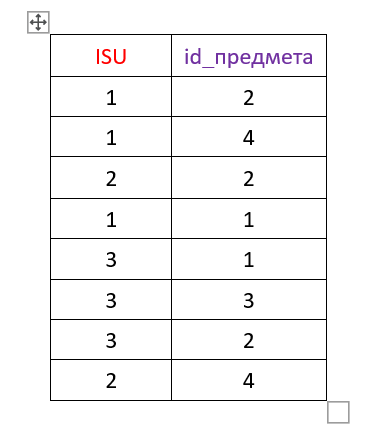
\includegraphics[width=0.7\textwidth]{pic/911.png}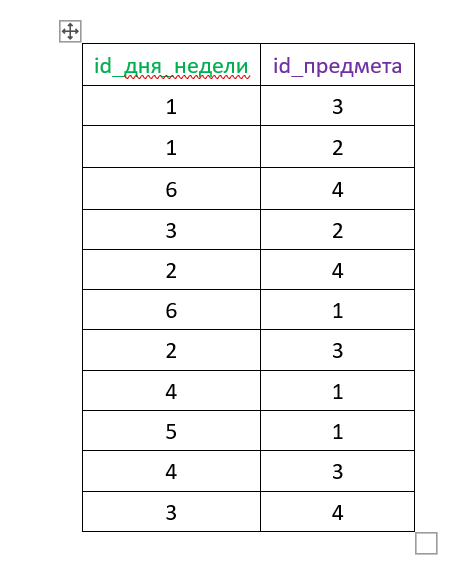
\includegraphics[width=0.7\textwidth]{pic/912.png} }
\end{minipage}
\end{figure}

В базе данных расписания ИТМО есть 2 таблицы:
\begin{itemize}
    \item В таблице 1 (рис. 1) каждому студенту по его номеру ИСУ сопоставлены предметы по их id. У одного номера ИСУ (студента) может быть много предметов, при этом на один предмет может ходить несколько студентов.
    \item В таблице 2 (рис. 2) каждому дню недели по его id (порядковый номер: 1-пн, 2-вт, 3-ср и т. д.) сопоставлены предметы по их id. В один день могут проводиться пары по нескольким предметам, при этом пары по одному предмету могут проходить несколько дней в неделе.
\end{itemize}
От Васи требуется по имеющимся данным вывести все возможные кортежи вида:

\begin{center}(номер ИСУ, день когда у этого студента есть пары)\end{center}

Например, ответ вида $\{(1, 1), (1, 5), (2, 1)\}$ будет означать что студент с ISU №1 имеет пары в понедельник и пятницу, а студент с ISU №2 имеет пары только в понедельник.

Помогите Васе решить данную задачу, используя ваши знания по дискретной математике.

---------------

Автор -- Тимур Гонтарь, М3206